% Historical text retained outside the canonical input closure.
\subsection{Actual gaps and the case register}
\label{subsec:trace-exact-ab-envelopes}

For an actual gap on \(e_{i,i+1}\), the definition from
\zcref{lem:gap-exhaustion} gives exactly
\[
 J_i=X_i([B_i,1-A_{i+1}]).
\]
This remains a closed singleton when \(B_i=1-A_{i+1}\).  Equivalently,
\[
 U_i\cap e_{i,i+1}=X_i([0,B_i)),
 \qquad
 U_{i+1}\cap e_{i,i+1}=X_i((1-A_{i+1},1]).
\]
Thus every point of \(J_i\), including its endpoints, is center-forced under
the skeleton-cover hypothesis.

\begin{figure}[!htbp]
\centering
\resizebox{.98\linewidth}{!}{%
\begin{tikzpicture}[
  x=1cm,y=1cm,>=Latex,
  route/.style={draw=black!35,rounded corners=2pt,align=center,
    minimum height=.78cm,text width=3.15cm,font=\scriptsize,fill=black!2},
  terminal/.style={draw=RadialTeal,rounded corners=2pt,align=center,
    minimum height=.78cm,text width=3.15cm,font=\scriptsize,fill=RadialTeal!7},
  lead/.style={-{Stealth[length=1.8mm]},draw=black!55,line width=.65pt}
]
  \node[route,text width=2.75cm,fill=CenterBlue!8,draw=CenterBlue]
    (root) at (0,0) {finite-enclosure state};

  \node[route] (z)  at (-7.6,-1.65)
    {$N_{\rm gap}=0$, $N_+=1$\\all V triangles $\Vdzero$};
  \node[route] (o0) at (-3.8,-1.65)
    {one gap, $N_+=0$\\common local pair $(p,q)$};
  \node[route] (t)  at (0,-1.65)
    {two gaps, CE2\\common pair on $T_1,\ldots,T_5$};
  \node[route] (o1) at (3.8,-1.65)
    {one gap, $N_+=1$\\three transverse actual reaches};
  \node[route] (ex) at (7.6,-1.65)
    {T3-like or Vd exceptional role};

  \node[terminal] (zt) at (-7.6,-3.45)
    {$D_0,\ldots,D_5,Q_-,Q_0,Q_+$\\nine-point support-cap terminal};
  \node[terminal] (o0t) at (-3.8,-3.45)
    {$\mathcal D_{h(1-c_*)}$ plus the actual gap\\disk-plus-point terminal};
  \node[terminal] (tt) at (0,-3.45)
    {$3e<p,q<1-5e$\\$D_2$ or $D_4$ beyond the C exit};
  \node[terminal] (o1t) at (3.8,-3.45)
    {$K_{\rm tr}$: $O,M_0$, two gap endpoints,\\and only $P_2,P_3,P_4$};
  \node[terminal] (ext) at (7.6,-3.45)
    {common rescuer-tail budget, one-third\\radial bound, or replacement};

  \foreach \n in {z,o0,t,o1,ex}{\draw[lead] (root) -- (\n);}
  \draw[lead] (z)--(zt);
  \draw[lead] (o0)--(o0t);
  \draw[lead] (t)--(tt);
  \draw[lead] (o1)--(o1t);
  \draw[lead] (ex)--(ext);

  \node[figlabel,align=center,text=black!60] at (0,-4.45)
    {The simplified routes retain only the support data used by their terminal.};
\end{tikzpicture}%
}
\caption{Roadmap of the simplified finite-enclosure chapter.  The one-gap
all-Vd0 witness uses only three transverse radial endpoints; the two-gap
terminal uses the interval $3e<p,q<1-5e$; and the T3-like and Vd1 paths share
one rescuer-tail lemma.}
\label{fig:finite-enclosure-roadmap}
\end{figure}

\begin{figure}[!htbp]
\centering
\begin{minipage}[t]{.32\linewidth}
\centering
\resizebox{\linewidth}{!}{%
\begin{tikzpicture}[x=5.2cm,y=1cm,>=Latex]
  \node[panellabel,anchor=west] at (0,1.35) {(a) actual open traces};
  \draw[line width=.75pt] (0,0)--(1,0);
  \draw[actualreach] (0,.06)--(.31,.06);
  \draw[actualreach] (.72,-.06)--(1,-.06);
  \draw[gap] (.31,0)--(.72,0);
  \fill (0,0) circle (.018) node[below=3pt,figlabel] {$V_i$};
  \fill (1,0) circle (.018) node[below=3pt,figlabel] {$V_{i+1}$};
  \draw[VertexOrange,fill=white,line width=.7pt] (.31,0) circle (.026);
  \fill[CenterBlue] (.31,0) circle (.011);
  \draw[VertexOrange,fill=white,line width=.7pt] (.72,0) circle (.026);
  \fill[CenterBlue] (.72,0) circle (.011);
  \node[figlabel,above] at (.31,.12) {$X_i(\ell)$};
  \node[figlabel,above] at (.72,.12) {$X_i(r)$};
  \node[figlabel,align=center] at (.5,-.62)
    {$U_i:\ [0,\loll)$\qquad$U_{i+1}:\ (r,1]$\\
     $J_i=[X_i(\ell),X_i(r)]\subset U_C$};
  \draw[flow] (.12,.82)--(.28,.82);
  \node[figlabel,anchor=west] at (.31,.82) {coordinate $t:0\to1$};
\end{tikzpicture}%
}
\end{minipage}\hfill
\begin{minipage}[t]{.32\linewidth}
\centering
resizebox{\linewidth}{!}{%
\begin{tikzpicture}[x=1cm,y=1cm,>=Latex]
  \node[panellabel,anchor=west] at (-.15,2.95) {(b) source-conditioned union};
  \coordinate (V) at (0,0);
  \draw[black!45,line width=.7pt] (V)--(3.2,0);
  \draw[black!45,line width=.7pt] (V)--(1.6,2.77);
  \fill[VertexOrange!14]
    (0,0)--(2.55,0).. controls (2.05,.65) and (1.68,1.25)..(1.05,1.82)--cycle;
  \fill[CenterBlue!12]
    (0,0)--(1.05,1.82).. controls (1.45,1.65) and (2.05,1.15)..(2.55,0)--cycle;
  \draw[VertexOrange,line width=.95pt]
    (2.55,0).. controls (2.05,.65) and (1.68,1.25)..(1.05,1.82);
  \draw[CenterBlue,line width=.95pt]
    (1.05,1.82).. controls (1.45,1.65) and (2.05,1.15)..(2.55,0);
  \node[figlabel,text=VertexOrange,align=center] at (2.32,.45)
    {$\mathcal E_i^{\rightarrow}$\\fixed actual endpoint};
  \node[figlabel,text=CenterBlue,align=center] at (1.13,1.17)
    {$\mathcal E_{i+1}^{\leftarrow}$};
  \begin{scope}[shift={(3.72,.15)},scale=.62]
    \draw[black!45] (0,0)--(2.4,0)--(1.2,2.08)--cycle;
    \draw[GapPurple,dashed,line width=1pt] (-.1,.72)--(2.5,.72);
    \draw[DemandRed,line width=1.3pt] (.25,.3)--(2.15,1.78);
    \draw[DemandRed,line width=1.2pt] (.3,1.8)--(2.1,.1);
    \node[DemandRed,font=\Large] at (1.2,1.03) {$\times$};
    \node[figlabel,align=center] at (1.2,-.45)
      {not a half-plane clip};
  \end{scope}
\end{tikzpicture}%
}
\end{minipage}\hfill
\begin{minipage}[t]{.32\linewidth}
\centering
\resizebox{\linewidth}{!}{%
\begin{tikzpicture}[x=1cm,y=1cm,>=Latex]
  \node[panellabel,anchor=west] at (-.25,2.95) {(c) equilateral support gauge};
  \fill[black!7]
    (-.35,.05)--(.25,-.35)--(1.1,-.18)--(1.48,.52)--(.75,1.32)--(-.15,1.05)--cycle;
  \draw[black!65,line width=.8pt]
    (-.35,.05)--(.25,-.35)--(1.1,-.18)--(1.48,.52)--(.75,1.32)--(-.15,1.05)--cycle;
  \node[figlabel] at (.55,.48) {$K$};
  \draw[CenterBlue,line width=1pt]
    (-1.05,-.85)--(2.08,-.32)--(.06,2.12)--cycle;
  \draw[flow] (.15,2.25)--(.15,2.75) node[above,figlabel] {$n$};
  \draw[flow] (2.1,-.42)--(2.55,-.68) node[right,figlabel] {$\mathsf Rn$};
  \draw[flow] (-1.02,-.95)--(-1.38,-1.28) node[left,figlabel] {$\mathsf R^2n$};
  \draw[black!35,dashed] (.75,1.32)--(.15,2.25);
  \draw[black!35,dashed] (1.48,.52)--(2.1,-.42);
  \draw[black!35,dashed] (-.35,.05)--(-1.02,-.95);
  \node[figlabel,align=center] at (.5,-1.43)
    {$\displaystyle \Lambda(K)=\frac1h\min_{\lVert n\rVert=1}
      \sum_{j=0}^{2}h_K(\mathsf R^jn)$};
\end{tikzpicture}%
}
\end{minipage}
\caption{Three conventions used throughout the finite-enclosure argument.
(a) A hollow outer marker records nonmembership in an open V trace, while the
filled center marker records selection of the same endpoint as a center-forced
witness.  (b) A trace-exact envelope is obtained by restricting the source
family to the prescribed actual maximal reach and then taking its union; it is
not an affine half-plane clipping.  (c) Equilateral enclosure is measured by
three support directions separated by $120^\circ$.  Incidences and interval
orders are exact; lengths are schematic.}
\label{fig:trace-exact-semantics-and-gauge}
\end{figure}


For the one-Vd rows define the normalized indices by
\[
 \{\sigma\}:=\{i\in\mathbb Z/6\mathbb Z:A_i+B_i>1\},
\]
\[
 \{\tau\}:=
 \{i\in\mathbb Z/6\mathbb Z:
 (o(T_i),n(T_i))\in\{(1,1),(1,2)\}\}.
\]
Rows A--E and the replacement router assume
\(S\subseteq U_C\cup\bigcup_{i=0}^5U_i\); row F assumes the hypothetical
cover of \(H\).

\begingroup
\small
\renewcommand{\arraystretch}{1.12}
\setlength{\tabcolsep}{1.5pt}
\begin{longtable}{@{}p{.19\textwidth}p{.17\textwidth}p{.36\textwidth}>{\raggedright\arraybackslash}p{.22\textwidth}@{}}
\caption{Exact finite-enclosure case register.  The symbolic columns determine
the row; the final column gives its concise geometric route.}
\label{tab:finite-enclosure-subcases}\\
\toprule
\shortstack[l]{gap\\conditions}&
\shortstack[l]{actual\\reaches}&
\shortstack[l]{role and\\placement}&route\\
\midrule
\endfirsthead
\toprule
\shortstack[l]{gap\\conditions}&
\shortstack[l]{actual\\reaches}&
\shortstack[l]{role and\\placement}&route\\
\midrule
\endhead
\(\begin{gathered}
N_{\rm gap}=1\\
J=J_0\\
J_0=X_0([\ell,r])\\
0<\ell\le r<1
\end{gathered}\)&
\(N_+=0\)&
\(\begin{gathered}
d=0\\
t\in\{0,1,2\}\\
N_E(T_C)\in\{1,2\}
\end{gathered}\)&
\textbf{A.} Complementary gap.\\[2pt]

\(N_{\rm gap}=2\)&
\(\begin{gathered}
N_+\in\{0,1\}\\
N_++t\le2\\
N_+t=0
\end{gathered}\)&
\(\begin{gathered}
d=0\\
N_E(T_C)=2\\
T_C\cap\{M_i\}_{i=0}^5=\{M_0\}
\end{gathered}\)&
\textbf{B.} CE2 short ray.\\[2pt]

\(\begin{gathered}
N_{\rm gap}=1\\
J=J_0\\
J_0=X_0([\ell,r])\\
0<\ell\le r<1
\end{gathered}\)&
\(\begin{gathered}
N_+=1\\
A_0+B_0>1
\end{gathered}\)&
\(\begin{gathered}
(d,t)=(0,0)\\
N_E(T_C)\in\{1,2\}\\
T_C\cap\{M_i\}_{i=0}^5=\{M_0\}
\end{gathered}\)&
\textbf{C.} Transverse seven-point witness.\\[2pt]

\(N_{\rm gap}\in\{1,2\}\)&
\(N_+=1\)&
\(\begin{gathered}
(d,t)=(0,1)\\
(o(T_0),n(T_0))=(2,1)\\
N_E(T_C)\in\{1,2\}\\
T_C\cap\{M_i\}_{i=0}^5=\{M_0\}
\end{gathered}\)&
\textbf{D$_T$.} T3-like supported tail.\\[2pt]

\(N_{\rm gap}\in\{1,2\}\)&
\(\begin{gathered}
N_+=1\\
A_0+B_0<1/2
\end{gathered}\)&
\(\begin{gathered}
(d,t)=(1,0)\\
(o(T_0),n(T_0))=(1,1)\\
N_E(T_C)=2\\
T_C\cap\{M_i\}_{i=0}^5=\{M_0\}
\end{gathered}\)&
\textbf{D$_V$.} Vd1 supported tail.\\[2pt]

\(N_{\rm gap}\in\{1,2\}\)&
\(N_+=1\)&
\(\begin{gathered}
(d,t)=(1,0)\\
\sigma=0\\
\tau\in\{1,5\}\\
N_E(T_C)=2\\
T_C\cap\{M_i\}_{i=0}^5=\{M_0\}
\end{gathered}\)&
\textbf{E$_a$.} Adjacent radial separation.\\[2pt]

\(N_{\rm gap}\in\{1,2\}\)&
\(N_+=1\)&
\(\begin{gathered}
(d,t)=(1,0)\\
\sigma=0\\
\tau\in\{2,3,4\}\\
N_E(T_C)=2\\
T_C\cap\{M_i\}_{i=0}^5=\{M_0\}
\end{gathered}\)&
\textbf{E$_n$.} Nonadjacent radial separation.\\[2pt]

\(N_{\rm gap}=0\)&
\(N_+=1\)&
\(\begin{gathered}
d+t\le6\\
H\subseteq U_C\cup\bigcup_{i=0}^5U_i
\end{gathered}\)&
\textbf{F.} Zero-gap nine-point obstruction.\\[2pt]

\(N_{\rm gap}\in\{1,2\}\)&
\(N_+=1\)&
\(\begin{gathered}
(d,t)=(1,0)\\
\sigma\in\{1,2,3,4,5\}\\
\tau\in\{1,2,3,4,5\}\\
\sigma\ne\tau\\
\sigma-\tau\equiv\pm1\pmod6\\
\bigl(o(T_\tau),n(T_\tau)\bigr)=(1,1)\\
M_\sigma\in T_\tau\\
N_E(T_C)=2\\
T_C\cap\{M_i\}_{i=0}^5=\{M_0\}
\end{gathered}\)&
\textbf{R.} Vd1 two-chart replacement; route by \(N'_{\rm gap}\).\\
\bottomrule
\end{longtable}
\endgroup

The short names in the last column are navigation aids.  The exact
hypotheses and witnesses below are the mathematical interfaces.

\subsection{Complementary gap and CE2 short ray}

\begin{lemma}[One-gap common-pair adapter]
\label{lem:new-one-gap-common-pair-adapter}
Under the exact row-A hypotheses, rotate the actual gap to
\[
 J_0=X_0([\ell,r]),
 \qquad
 \ell=B_0,
 \qquad
 r=1-A_1,
\]
and put
\[
 p:=1-r,
 \qquad
 q:=\ell.
\]
Then
\[
 \forall i\in\mathbb Z/6\mathbb Z,
 \quad
 (p\le A_i\ \land\ q\le B_i)
 \ \lor
 (q\le A_i\ \land\ p\le B_i).
\]
\end{lemma}

\begin{proof}
The exact five-handoff calculation is
\zcref{lem:appendix-one-gap-common-pair-adapter}.
\end{proof}

Let
\[
 0<p,q<1,
 \qquad
 p+q\le1,
 \qquad
 c_*:=c_{\max}(p,q),
\]
and put
\[
 J(p,q):=X_0([q,1-p]),
 \qquad
 \mathcal D(p,q):=\mathbb B(O,h(1-c_*)).
\]

\begin{theorem}[Complementary-gap enclosure]
\label{thm:new-complementary-gap}
\[
 \Lambda\bigl(\mathcal D(p,q)\cup J(p,q)\bigr)\ge1.
\]
The conclusion includes \(p+q=1\), when \(J(p,q)\) is a singleton.
\end{theorem}

\begin{figure}[!htbp]
\centering
\begin{minipage}[t]{.315\linewidth}
\centering
\resizebox{\linewidth}{!}{%
\begin{tikzpicture}[scale=2.15,>=Latex]
  \node[panellabel,anchor=west] at (-1.05,1.16) {(a) the complementary gap};
  \HexCoords
  \DrawHexagon
  \draw[ray] (O)--($(V0)!.25!(V1)$);
  \coordinate (G) at ($(V0)!.25!(V1)$);
  \coordinate (H) at ($(V0)!.67!(V1)$);
  \draw[gap] (G)--(H);
  \fill[DemandRed] (G) circle (.025) node[right=2pt,figlabel] {$G=X(q)$};
  \fill[GapPurple] (H) circle (.021) node[left=2pt,figlabel] {$X(1-p)$};
  \draw[DemandRed,line width=.85pt] (O)--(G);
  \node[figlabel,align=center] at (0,-1.16)
    {$m=\min\{p,q\}$, choose the farther endpoint $G$\\
     $\lVert G\rVert^2=1-m+m^2$};
\end{tikzpicture}%
}
\end{minipage}\hfill
\begin{minipage}[t]{.335\linewidth}
\centering
\resizebox{\linewidth}{!}{%
\begin{tikzpicture}[scale=2.15,>=Latex]
  \node[panellabel,anchor=west] at (-1.08,1.16) {(b) six radial witnesses};
  \HexCoords
  \DrawHexagon
  \DrawRays
  \foreach \i in {0,...,5}{
    \coordinate (D\i) at ($(O)!.18!(V\i)$);
    \fill[DemandRed] (D\i) circle (.024);
  }
  \draw[DemandRed!65,line width=.75pt]
    (D0)--(D1)--(D2)--(D3)--(D4)--(D5)--cycle;
  \draw[CenterBlue,dashed,fill=CenterBlue!7,line width=.8pt]
    (O) circle ({.18*sqrt(3)/2});
  \node[figlabel,right] at (D0) {$D_0=dV_0$};
  \node[figlabel,above right] at (D1) {$D_1$};
  \node[figlabel,align=center] at (0,-1.16)
    {$d=1-c_*$, $c_*=c_{\max}(p,q)$\\
     $\mathcal D_{hd}\subset\operatorname{conv}\{D_0,\ldots,D_5\}$};
\end{tikzpicture}%
}
\end{minipage}\hfill
\begin{minipage}[t]{.315\linewidth}
\centering
\resizebox{\linewidth}{!}{%
\begin{tikzpicture}[x=2.25cm,y=2.25cm,>=Latex]
  \node[panellabel,anchor=west] at (-.72,1.02) {(c) enclosure terminal};
  \coordinate (O) at (0,0);
  \coordinate (G) at (1.02,.31);
  \draw[CenterBlue!35,fill=CenterBlue!8,line width=.8pt] (O) circle (.24);
  \fill[DemandRed] (G) circle (.023) node[right=2pt,figlabel] {$G$};
  \draw[black,line width=1pt]
    (-.42,-.64)--(1.18,-.18)--(.05,1.08)--cycle;
  \draw[DemandRed,dashed,line width=.75pt] (O)--(G);
  \node[figlabel] at (.03,-.08) {$\mathcal D_{hd}$};
  \node[figlabel,align=center] at (.23,-1.03)
    {$\displaystyle
      \Lambda\!\left(\mathcal D_{hd}\cup\{G\}\right)\ge1$\\
     hence $\Lambda(\{D_0,\ldots,D_5,G\})\ge1$};
\end{tikzpicture}%
}
\end{minipage}
\caption{The complementary-gap enclosure mechanism.  The farther endpoint
$G$ of $J(p,q)$ is center-forced.  Common-pair domination produces the six
center-forced points $D_i=(1-c_*)V_i$, whose convex hull contains the disk
$\mathcal D_{h(1-c_*)}$.  The disk-plus-point formula then forces enclosing
side length at least one.  The disk is not an additional witness; it is
contained in the convex hull of the six finite radial witnesses.}
\label{fig:complementary-gap-certificate}
\end{figure}


\begin{proof}
The enclosure optimization, including the disk--point transition, is
\zcref{lem:new-disk-point-formula,lem:appendix-complementary-gap}.
\end{proof}

In the six case figures below, orange marks actual gaps, purple marks sampled
finite-enclosure points, and the dashed red line is an enclosing triangle.
The shading and the displayed triangle are illustrative, not proof objects.

\begin{figure}[!htbp]
\centering
\begin{minipage}[t]{.485\linewidth}
\centering
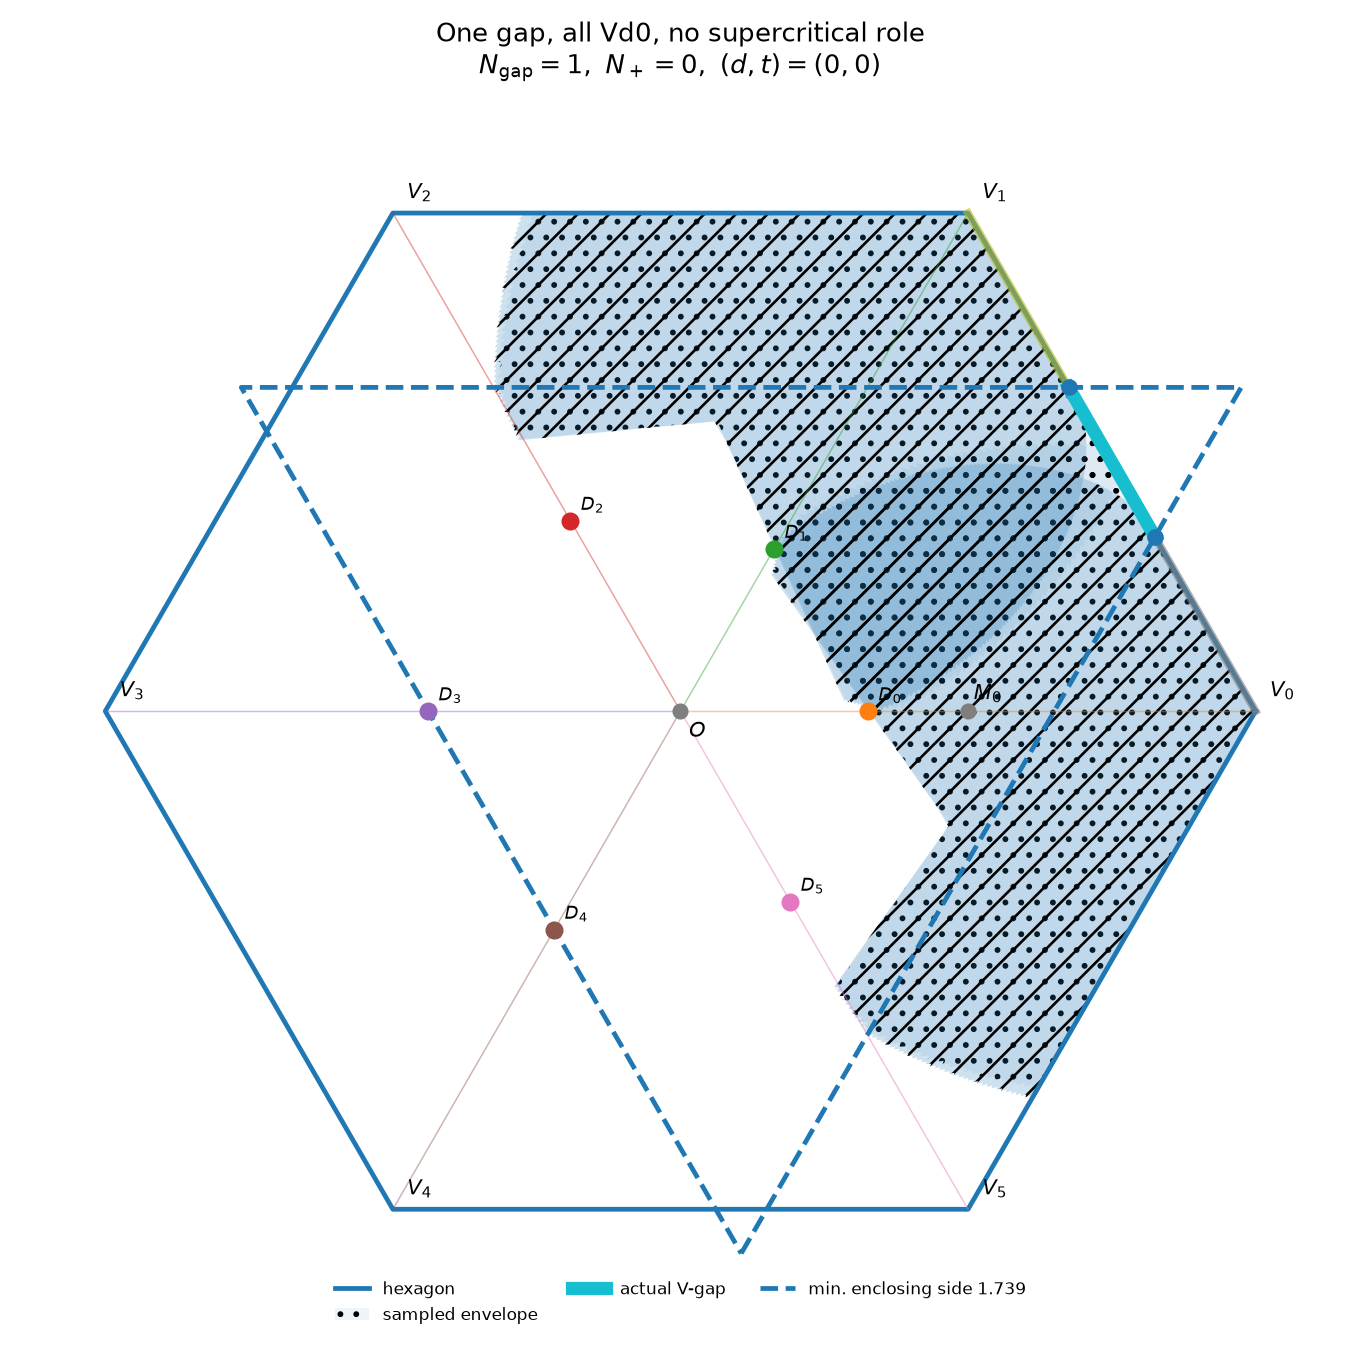
\includegraphics[width=\linewidth]
  {figures/trace_exact_ab/one_gap_n0_vd0.png}
\par\smallskip
\textbf{All \(\Vdzero\).}\par\smallskip
{\footnotesize
\(\begin{gathered}
N_{\rm gap}=1\\
N_+=0\\
(d,t)=(0,0)
\end{gathered}\)}
\end{minipage}\hfill
\begin{minipage}[t]{.485\linewidth}
\centering
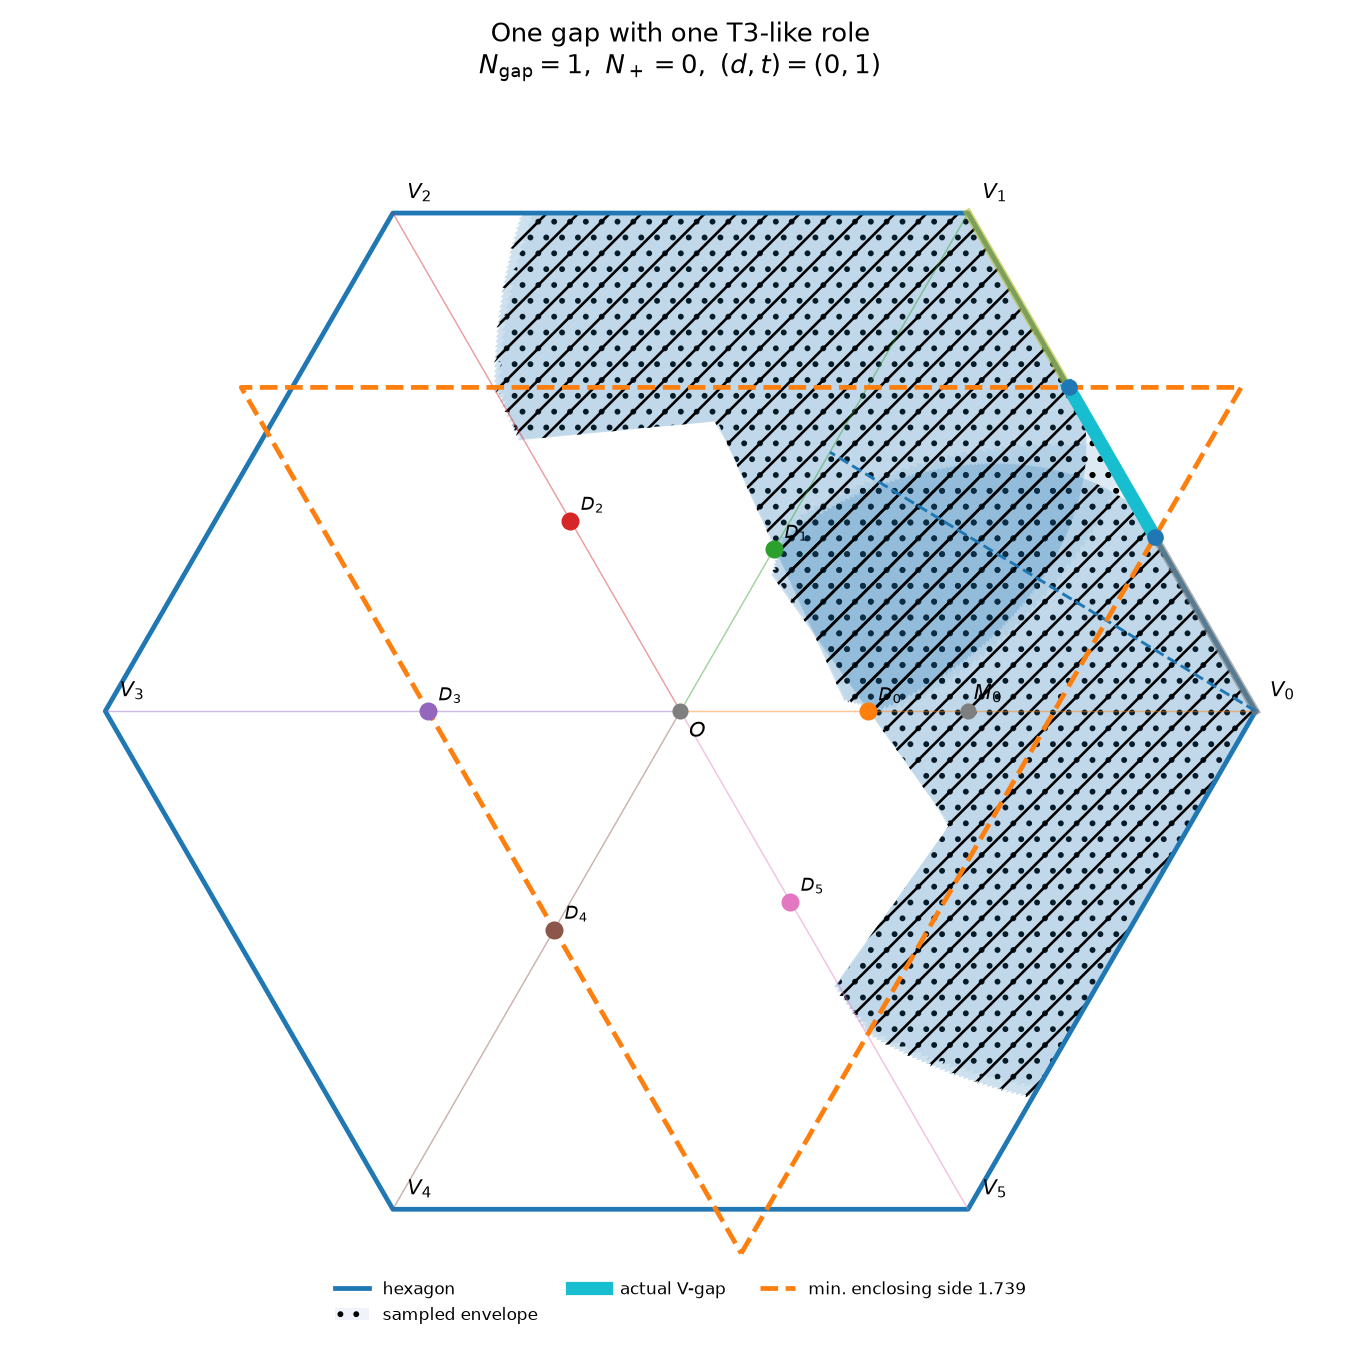
\includegraphics[width=\linewidth]
  {figures/trace_exact_ab/one_t3_n0.png}
\par\smallskip
\textbf{One \(\Tlike\) role.}\par\smallskip
{\footnotesize
\(\begin{gathered}
N_{\rm gap}=1\\
N_+=0\\
(d,t)=(0,1)
\end{gathered}\)}
\end{minipage}

\par\medskip
\begin{minipage}[t]{.485\linewidth}
\centering
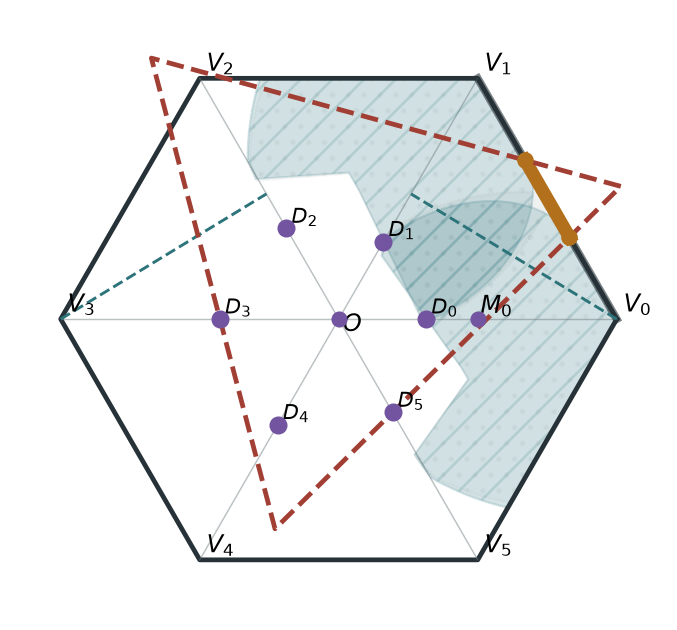
\includegraphics[width=\linewidth]
  {figures/trace_exact_ab/two_t3_n0.png}
\par\smallskip
\textbf{Two \(\Tlike\) roles.}\par\smallskip
{\footnotesize
\(\begin{gathered}
N_{\rm gap}=1\\
N_+=0\\
(d,t)=(0,2)
\end{gathered}\)}
\end{minipage}
\caption{Case A: sampled complementary-gap data.}
\label{fig:finite-enclosure-case-a-examples}
\end{figure}

\FloatBarrier

In the CE2 two-gap normalization, define the two positive C-trace endpoints
geometrically by
\[
 p:=\min\{x\in[0,1]:X_5(x)\in T_C\},
\]
\[
 q:=1-\max\{x\in[0,1]:X_0(x)\in T_C\},
\]
and put
\[
 c_*:=c_{\max}(p,q),
 \qquad
 D_2:=(1-c_*)V_2,
 \qquad
 D_4:=(1-c_*)V_4.
\]

\begin{lemma}[Two-gap common-pair adapter]
\label{lem:new-two-gap-common-pair-adapter}
Under the exact row-B hypotheses,
\[
 \forall i\in\{1,2,3,4,5\},
 \quad
 (p\le A_i\ \land\ q\le B_i)
 \ \lor
 (q\le A_i\ \land\ p\le B_i).
\]
For \(j\in\mathbb Z/6\mathbb Z\), if \((o(T_j),n(T_j))=(2,1)\) and
\(\Haus\bigl(T_j\cap(r_2\cup r_4)\bigr)>0\), then
\[
 A_j+B_j\le1,
 \qquad
 \max\{C_+(A_j,B_j),C_-(A_j,B_j)\}\le c_*.
\]
\end{lemma}

\begin{proof}
The exact two-gap handoff calculation and the T3-like capacity check are
\zcref{lem:appendix-two-gap-common-pair-adapter,
lem:new-common-pair-domination}.
\end{proof}

\begin{theorem}[CE2 short-ray obstruction]
\label{thm:new-ce2-short-ray}
Assume
\[
 N_E(T_C)=2,
 \qquad
 N_{\rm gap}=2,
 \qquad
 N_+\in\{0,1\},
 \qquad
 d=0,
 \qquad
 N_++t\le2.
\]
If every \(i\in\{1,2,3,4,5\}\) has either
\[
 p\le A_i,\qquad q\le B_i,
\]
or
\[
 q\le A_i,\qquad p\le B_i,
\]
then
\[
 D_2,D_4\in U_C,
 \qquad
 \{D_2,D_4\}\nsubseteq T_C.
\]
\end{theorem}

\begin{figure}[!htbp]
\centering
\begin{minipage}[t]{.31\linewidth}
\centering
\resizebox{\linewidth}{!}{%
\begin{tikzpicture}[scale=2.1,>=Latex]
  \node[panellabel,anchor=west] at (-1.08,1.18) {(a) two CE2 gaps};
  \HexCoords
  \DrawHexagon
  \DrawRays
  \draw[gap] ($(V0)!.18!(V1)$)--($(V0)!.36!(V1)$);
  \draw[gap] ($(V5)!.64!(V0)$)--($(V5)!.84!(V0)$);
  \draw[centerrole]
    (.07,.03)--(.45,.54)--(.62,-.35)--cycle;
  \node[figlabel,text=GapPurple] at (.55,.69) {demand $q$};
  \node[figlabel,text=GapPurple] at (.78,-.58) {demand $p$};
  \node[figlabel,align=center] at (0,-1.18)
    {$p,q$ are the common\\boundary demands};
\end{tikzpicture}%
}
\end{minipage}\hfill
\begin{minipage}[t]{.37\linewidth}
\centering
\resizebox{\linewidth}{!}{%
\begin{tikzpicture}[x=5cm,y=1cm,>=Latex]
  \node[panellabel,anchor=west] at (-.02,2.45) {(b) transverse center exits};
  \draw[flow] (0,1.55)--(1,1.55);
  \draw[flow] (0,.35)--(1,.35);
  \fill (0,1.55) circle (.018) node[left=2pt,figlabel] {$O$};
  \fill (1,1.55) circle (.018) node[right=2pt,figlabel] {$V_2$};
  \fill (0,.35) circle (.018) node[left=2pt,figlabel] {$O$};
  \fill (1,.35) circle (.018) node[right=2pt,figlabel] {$V_4$};
  \coordinate (E2) at (.08,1.55);
  \coordinate (D2) at (.14,1.55);
  \coordinate (D4) at (.14,.35);
  \coordinate (E4) at (.19,.35);
  \fill[CenterBlue] (E2) circle (.024) node[above=3pt,figlabel] {C trace end};
  \fill[DemandRed] (D2) circle (.024) node[below=3pt,figlabel] {$D_2$};
  \fill[DemandRed] (D4) circle (.024) node[above=3pt,figlabel] {$D_4$};
  \fill[CenterBlue] (E4) circle (.024) node[below=3pt,figlabel] {C trace end};
  \draw[GapPurple,line width=1.1pt] (E2)--(D2);
  \draw[black!35,line width=1.1pt] (D4)--(E4);
  \node[figlabel,align=center] at (.52,-.42)
    {one radial witness lies beyond the corresponding C trace};
\end{tikzpicture}%
}
\end{minipage}\hfill
\begin{minipage}[t]{.28\linewidth}
\centering
\resizebox{\linewidth}{!}{%
\begin{tikzpicture}[x=4.5cm,y=1cm,>=Latex]
  \node[panellabel,anchor=west] at (-.04,2.42) {(c) the case split};
  \node[figlabel,anchor=west] at (0,1.84) {first radial alternative};
  \draw[line width=.65pt] (0,1.38)--(1,1.38);
  \fill (0,1.38) circle (.017) node[left=1pt,figlabel] {$O$};
  \fill[CenterBlue] (.22,1.38) circle (.023) node[above=2pt,figlabel] {C trace};
  \fill[DemandRed] (.43,1.38) circle (.023) node[below=2pt,figlabel] {$D_2$};
  \draw[GapPurple,line width=1pt] (.22,1.38)--(.43,1.38);
  \node[figlabel,anchor=west] at (0,.73) {second radial alternative};
  \draw[line width=.65pt] (0,.27)--(1,.27);
  \fill (0,.27) circle (.017) node[left=1pt,figlabel] {$O$};
  \fill[CenterBlue] (.22,.27) circle (.023) node[above=2pt,figlabel] {C trace};
  \fill[DemandRed] (.43,.27) circle (.023) node[below=2pt,figlabel] {$D_4$};
  \draw[GapPurple,line width=1pt] (.22,.27)--(.43,.27);
  \node[figlabel,align=center] at (.5,-.36)
    {the red point lies beyond\\the corresponding center exit};
\end{tikzpicture}%
}
\end{minipage}
\caption{The CE2 short-ray terminal.  The two boundary gaps determine the
common pair $(p,q)$ and the center-forced radial witnesses $D_2,D_4$.  The
theorem proves that at least one of these witnesses lies beyond the
corresponding C-triangle trace and is uncovered.  The displayed ordering is
schematic.}
\label{fig:ce2-short-ray-certificate}
\end{figure}


\begin{proof}
The first inclusion is type-aware radial forcing.  The signed CE2
optimization proving the final strict noncontainment is
\zcref{lem:appendix-ce2-short-ray}.
\end{proof}

\begin{figure}[!htbp]
\centering
\begin{minipage}[t]{.485\linewidth}
\centering
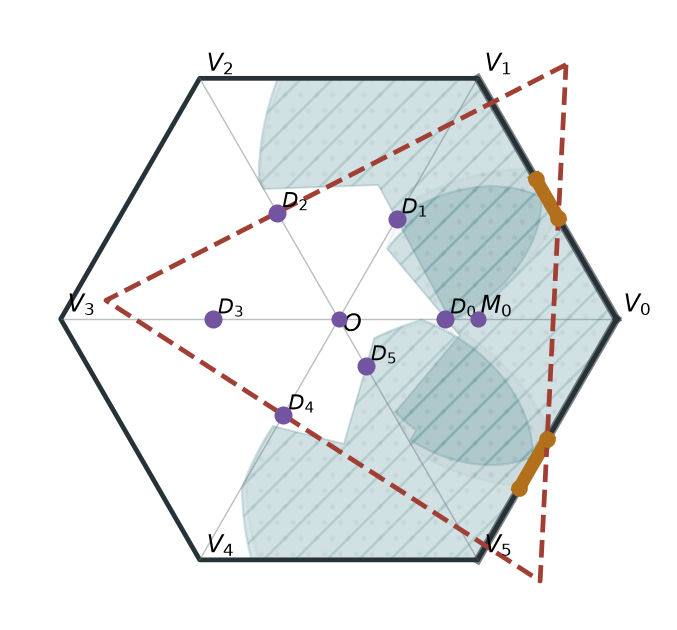
\includegraphics[width=\linewidth]
  {figures/trace_exact_ab/two_gap_vd0.png}
\par\smallskip
\textbf{All \(\Vdzero\).}\par\smallskip
{\footnotesize
\(\begin{gathered}
N_{\rm gap}=2\\
N_E(T_C)=2\\
N_+=0\\
(d,t)=(0,0)
\end{gathered}\)}
\end{minipage}\hfill
\begin{minipage}[t]{.485\linewidth}
\centering
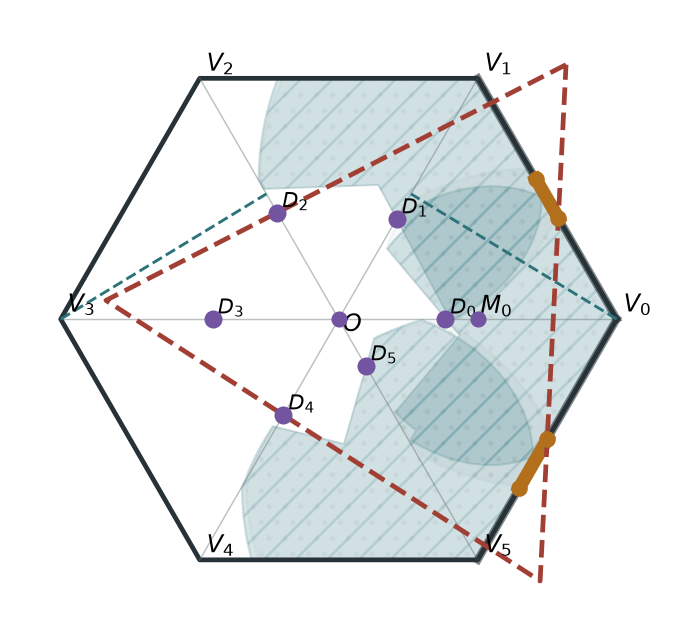
\includegraphics[width=\linewidth]
  {figures/trace_exact_ab/two_gap_t3_n0.png}
\par\smallskip
\textbf{Two \(\Tlike\) roles.}\par\smallskip
{\footnotesize
\(\begin{gathered}
N_{\rm gap}=2\\
N_E(T_C)=2\\
N_+=0\\
(d,t)=(0,2)
\end{gathered}\)}
\end{minipage}

\par\medskip
\begin{minipage}[t]{.485\linewidth}
\centering
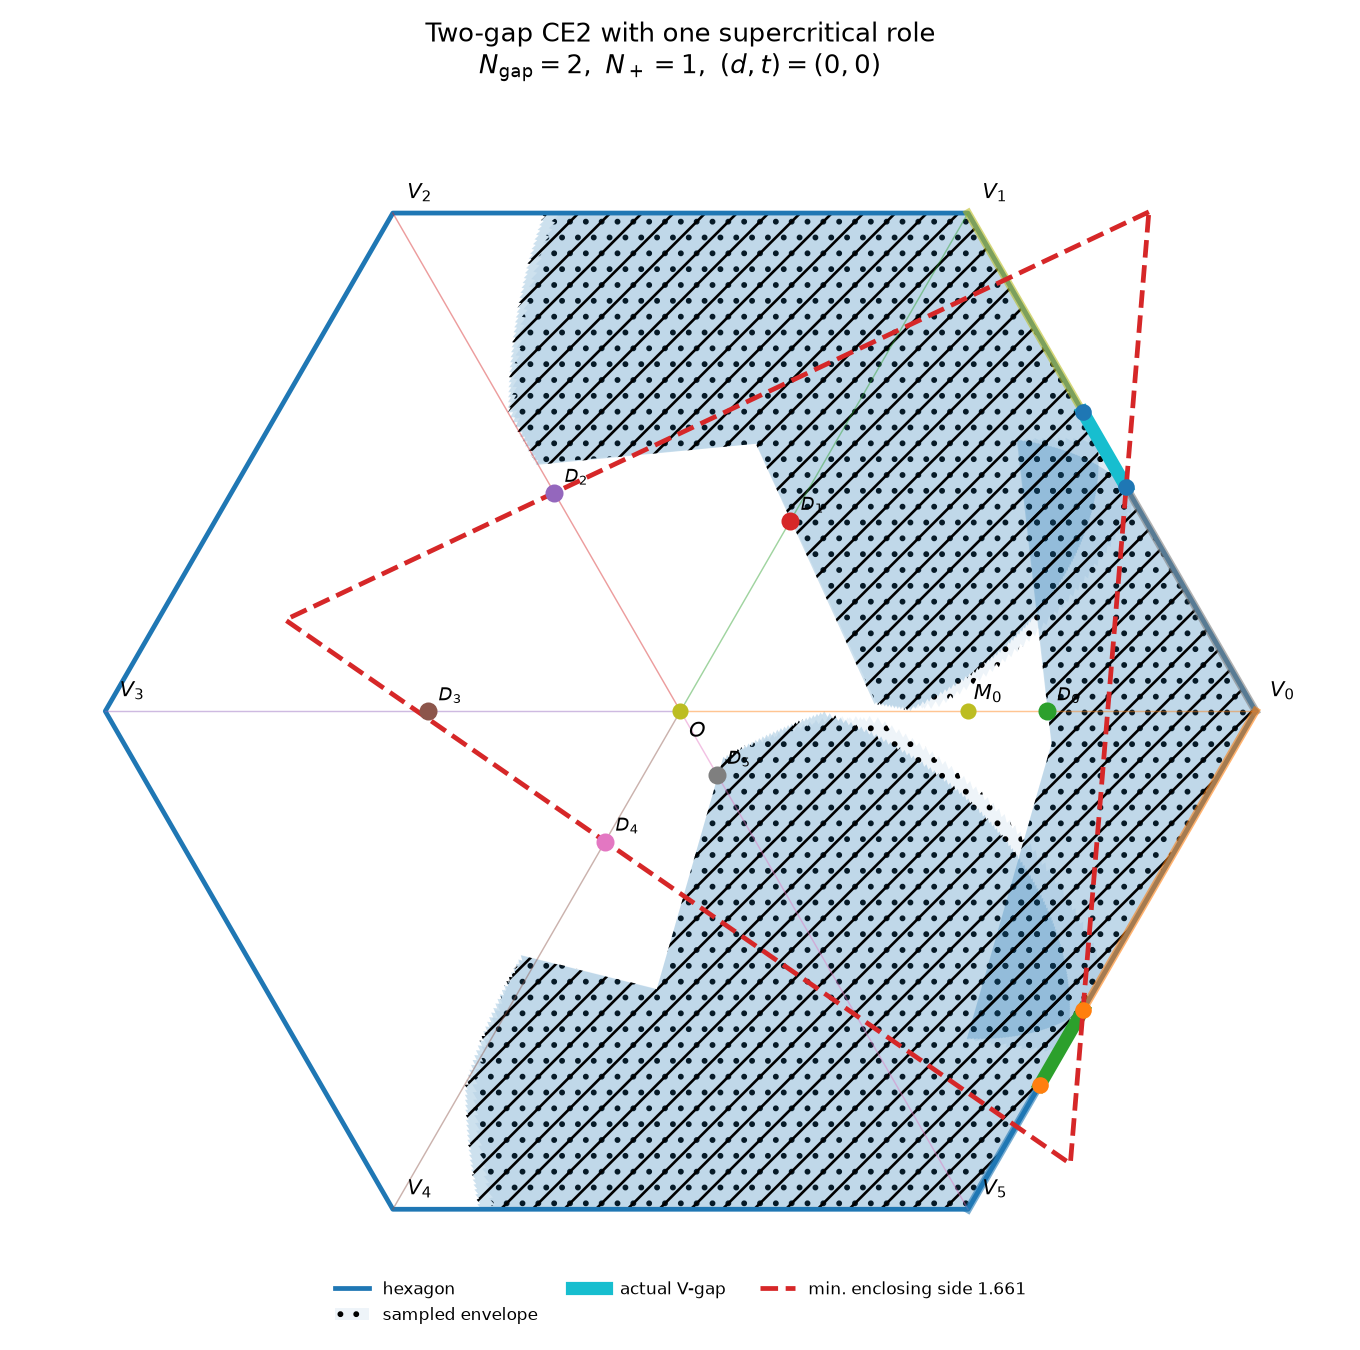
\includegraphics[width=\linewidth]
  {figures/trace_exact_ab/two_gap_n1_vd0.png}
\par\smallskip
\textbf{One supercritical role.}\par\smallskip
{\footnotesize
\(\begin{gathered}
N_{\rm gap}=2\\
N_E(T_C)=2\\
N_+=1\\
(d,t)=(0,0)
\end{gathered}\)}
\end{minipage}
\caption{Case B: sampled \(\CEtwo\) short-ray data.}
\label{fig:finite-enclosure-case-b-examples}
\end{figure}

\FloatBarrier

\begin{proposition}[The common-pair nonzero-gap closures]
\label{prop:new-nplus-zero-gap-closures}
Every row A or B of \zcref{tab:finite-enclosure-subcases} is impossible.
\end{proposition}

\begin{proof}
In row A, \zcref{lem:new-one-gap-common-pair-adapter}, type-aware radial
forcing, and common-pair domination put the six points
\((1-c_*)V_i\) in \(U_C\).  Their convex hull contains
\(\mathcal D(p,q)\), while the actual gap is \(J(p,q)\subset U_C\).
Now \zcref{thm:new-complementary-gap,lem:new-compact-open-shrink}
contradict each other.

In row B, \zcref{lem:new-two-gap-common-pair-adapter} supplies every
hypothesis of \zcref{thm:new-ce2-short-ray}.  That theorem puts both
\(D_2,D_4\) in \(U_C\subseteq T_C\) and at least one outside \(T_C\), a
contradiction.  This includes \(N_+=1\).
\end{proof}

\subsection{The transverse seven-point witness}

Normalize row C so that
\[
 J=J_0=X_0([\ell,r]),
 \qquad
 \ell:=B_0,
 \qquad
 r:=1-A_1,
 \qquad
 0<\ell\le r<1.
\]
For the actual radial reaches define
\[
 P_i:=(1-C_i)V_i,
\]
and define exactly
\[
 K_{\rm tr}:=
 \{O,M_0,X_0(\ell),X_0(r),P_2,P_3,P_4\}.
\]

\begin{lemma}[The transverse witness is center-forced]
\label{lem:readable-k410-forced}
Under the exact row-C hypotheses,
\[
 K_{\rm tr}\subset U_C.
\]
\end{lemma}

\begin{figure}[!htbp]
\centering
\begin{minipage}[t]{.325\linewidth}
\centering
\resizebox{\linewidth}{!}{%
\begin{tikzpicture}[scale=2.05,>=Latex]
  \node[panellabel,anchor=west] at (-1.08,1.18) {(a) the finite set $K_{410}$};
  \HexCoords
  \DrawHexagon
  \DrawRays
  \draw[gap] ($(V0)!.20!(V1)$)--($(V0)!.34!(V1)$);
  \def\rr{{.13,.19,.15,.10,.21,.16}}
  \foreach \i in {0,...,5}{
    \pgfmathparse{\rr[\i]}
    \coordinate (P\i) at ($(O)!{\pgfmathresult}!(V\i)$);
    \draw[VertexOrange,fill=white,line width=.65pt] (P\i) circle (.027);
    \fill[DemandRed] (P\i) circle (.012);
  }
  \fill[CenterBlue] (O) rectangle +(0.035,0.035);
  \fill[CenterBlue] ($(O)!.5!(V0)$) rectangle +(0.035,0.035);
  \fill[GapPurple] ($(V0)!.20!(V1)$) -- ++(.03,.02) -- ++(-.03,.02) -- ++(-.03,-.02) -- cycle;
  \fill[GapPurple] ($(V0)!.34!(V1)$) -- ++(.03,.02) -- ++(-.03,.02) -- ++(-.03,-.02) -- cycle;
  \node[figlabel,below left] at (O) {$O$};
  \node[figlabel,above] at ($(O)!.5!(V0)$) {$M_0$};
  \node[figlabel,right] at (P0) {$P_0=(1-C_0)V_0$};
  \node[figlabel,align=center] at (0,-1.18)
    {circles: actual radial endpoints $P_i$\\diamonds: $X(\ell),X(r)$};
\end{tikzpicture}%
}
\end{minipage}\hfill
\begin{minipage}[t]{.35\linewidth}
\centering
\resizebox{\linewidth}{!}{%
\begin{tikzpicture}[scale=2.05,>=Latex]
  \node[panellabel,anchor=west] at (-1.08,1.18) {(b) a candidate center triangle};
  \HexCoords
  \DrawHexagon
  \DrawRays
  \draw[centerrole]
    (-.58,-.32)--(.88,-.20)--(-.02,.86)--cycle;
  \coordinate (P0) at ($(O)!.13!(V0)$);
  \coordinate (E0) at ($(O)!.30!(V0)$);
  \draw[CenterBlue,line width=1pt] (O)--(E0);
  \draw[VertexOrange,line width=1.2pt] (V0)--(P0);
  \draw[VertexOrange,fill=white,line width=.65pt] (P0) circle (.027);
  \fill[DemandRed] (P0) circle (.012);
  \fill[CenterBlue] (E0) circle (.023);
  \node[figlabel,above] at (P0) {$P_i$};
  \node[figlabel,below] at (E0) {$E_i'=d_i'V_i$};
  \draw[dimline] ($(O)+(0,-.13)$)--($(P0)+(0,-.13)$)
    node[midway,below=1pt,figlabel] {$1-C_i$};
  \draw[dimline] ($(O)+(0,.13)$)--($(E0)+(0,.13)$)
    node[midway,above=1pt,figlabel] {$d_i'$};
  \node[figlabel,align=center] at (0,-1.18)
    {$P_i\in T_C'\Longrightarrow d_i'\ge1-C_i$\\
     equivalently $C_i\ge1-d_i'$};
\end{tikzpicture}%
}
\end{minipage}\hfill
\begin{minipage}[t]{.285\linewidth}
\centering
\resizebox{\linewidth}{!}{%
\begin{tikzpicture}[x=5cm,y=1cm,>=Latex]
  \node[panellabel,anchor=west] at (-.03,2.62) {(c) closing a boundary gap};
  \node[figlabel,anchor=west] at (0,2.14) {before};
  \draw[line width=.65pt] (0,1.70)--(1,1.70);
  \draw[actualreach] (0,1.76)--(.38,1.76);
  \draw[centertrace] (.53,1.64)--(.77,1.64);
  \draw[gap] (.38,1.70)--(.53,1.70);
  \node[figlabel,text=GapPurple] at (.455,1.98) {gap};
  \node[figlabel,anchor=west] at (0,1.08) {after $C_i\ge1-d_i'$};
  \draw[line width=.65pt] (0,.64)--(1,.64);
  \draw[actualreach] (0,.70)--(.58,.70);
  \draw[centertrace] (.53,.58)--(.77,.58);
  \draw[RadialTeal,line width=1pt] (.53,.64)--(.58,.64);
  \node[figlabel,text=RadialTeal] at (.555,.91) {overlap};
  \node[figlabel,align=center] at (.5,-.03)
    {every candidate gap closes\\$\Rightarrow$ CE1 or CE2 terminal};
\end{tikzpicture}%
}
\end{minipage}
\caption{The actual-reach mechanism behind the anisotropic set $K_{410}$.
The six points $P_i=(1-C_i)V_i$ retain the actual own-radial reaches rather
than a common relaxed radius.  If a candidate center triangle $T_C'$ contains
$K_{410}$, its exit $d_i'$ on every radial arm satisfies
$d_i'\ge1-C_i$, equivalently $C_i\ge1-d_i'$.  The corresponding V trace then
meets the center contribution and closes the associated boundary gap, forcing
the candidate into the CE1 or CE2 terminal used in the proof.  Lengths are
schematic; the order relations are exact.}
\label{fig:k410-actual-reach-certificate}
\end{figure}


\begin{proof}
The gap endpoints are missed by both incident open V triangles.  Each
\(P_i\) is the excluded endpoint of the actual closed radial trace; the Vd0
restriction excludes adjacent support, and diameter excludes nonlocal roles.
The midpoint belongs only to the C triangle.
\end{proof}

\begin{proposition}[CE2 transverse threshold terminal]
\label{prop:readable-k410-ce2}
For an open unit equilateral triangle \(U_C\), put
\(T_C:=\overline{U_C}\).  Then
\[
 N_E(T_C)=2\Longrightarrow K_{\rm tr}\nsubseteq U_C.
\]
\end{proposition}

\begin{proof}
The exact endpoint squeeze and the two transverse thresholds are proved in
\zcref{lem:readable-k410-upper-bound,lem:appendix-ktr-ce2}.
\end{proof}

\begin{proposition}[CE1 three-transverse return]
\label{prop:readable-k410-ce1}
For an open unit equilateral triangle \(U_C\), put
\(T_C:=\overline{U_C}\).  Then
\[
 N_E(T_C)=1\Longrightarrow K_{\rm tr}\nsubseteq U_C.
\]
\end{proposition}

\begin{proof}
The three actual endpoints \(P_2,P_3,P_4\) give the CE1 radial hypotheses;
the reverse-path calculation is \zcref{prop:new-ce1-direct-certificate}.
No radial point on \(r_0\) is used.
\end{proof}

\begin{proposition}[Transverse seven-point enclosure]
\label{prop:new-nplus-one-all-vd0}
Under the exact row-C hypotheses,
\[
 \Lambda(K_{\rm tr})\ge1.
\]
\end{proposition}

\begin{proof}
By \zcref{prop:ce-classification}, the closure of a candidate C triangle has
type \(\CEone\) or \(\CEtwo\).
The preceding two propositions exclude both possibilities, and
\zcref{lem:new-compact-open-shrink} gives the enclosure conclusion.
\end{proof}

\begin{figure}[!htbp]
\centering
\begin{minipage}[t]{.485\linewidth}
\centering
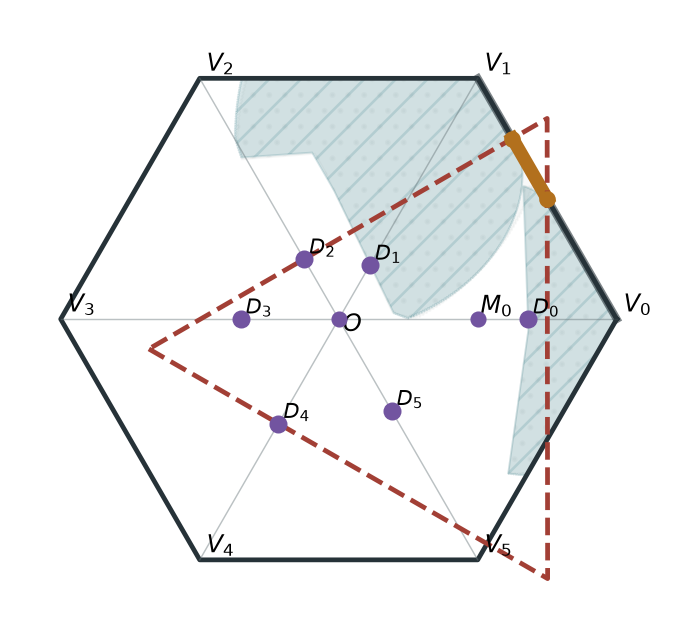
\includegraphics[width=\linewidth]
  {figures/trace_exact_ab/one_gap_n1_vd0_ce1.png}
\par\smallskip
\textbf{\(\CEone\) terminal context.}\par\smallskip
{\footnotesize
\(\begin{gathered}
N_{\rm gap}=1\\
N_+=1\\
(d,t)=(0,0)\\
N_E(T_C)=1
\end{gathered}\)}
\end{minipage}\hfill
\begin{minipage}[t]{.485\linewidth}
\centering
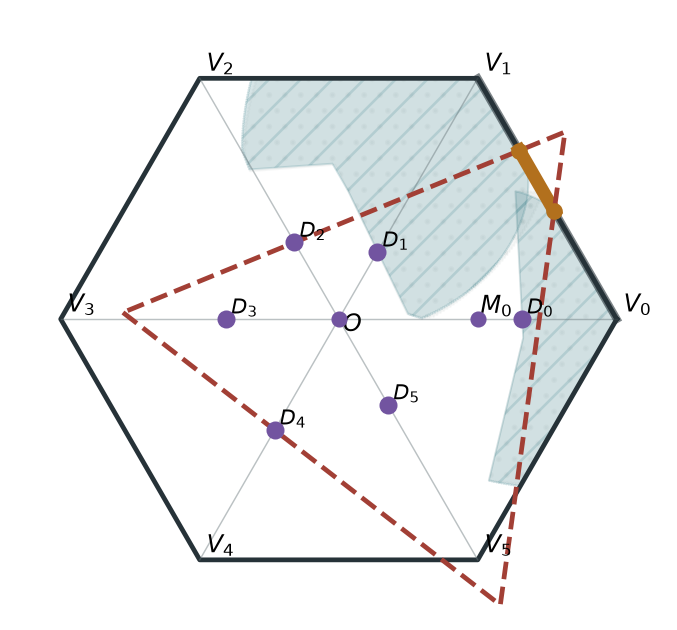
\includegraphics[width=\linewidth]
  {figures/trace_exact_ab/one_gap_n1_vd0_ce2.png}
\par\smallskip
\textbf{\(\CEtwo\) terminal context.}\par\smallskip
{\footnotesize
\(\begin{gathered}
N_{\rm gap}=1\\
N_+=1\\
(d,t)=(0,0)\\
N_E(T_C)=2
\end{gathered}\)}
\end{minipage}
\caption{Case C: sampled transverse-witness data.}
\label{fig:finite-enclosure-case-c-examples}
\end{figure}

\FloatBarrier

\subsection{Supported tails and radial separation}

For \(0\le c<1/2\), define
\[
 M_c^{\rm sup}:=
 \sup\{M_c(a):0\le a\le1,\ M_c(a)>1-a\},
\]
and set
\[
 M_{1/2}^{\rm sup}:=\frac12.
\]
The endpoint value is the continuous extension, not the supremum of an empty
strict feasible set.

Both supported-tail adapters use an actual interval
\[
 T_0\cap r_1=\{V_1+x(O-V_1):c\le x\le u\},
\]
\[
 0<c\le\frac12\le u<1,
 \qquad
 \varepsilon:=1-u,
 \qquad
 C_1\ge c.
\]
With \(M:=M_c^{\rm sup}\), their common exact conclusion is
\[
 \sum_{i=2}^5(A_i+B_i)\ge4+M-B_1>4.
\]

\begin{proposition}[T3-like supported-tail terminal]
\label{prop:new-one-t3-terminal}
Assume
\[
 N_{\rm gap}\in\{1,2\},
 \qquad
 N_+=1,
 \qquad
 (d,t)=(0,1),
 \qquad
 N_E(T_C)\in\{1,2\},
\]
\[
 T_C\cap\{M_0,\ldots,M_5\}=\{M_0\},
 \qquad
 (o(T_0),n(T_0))=(2,1),
\]
\[
 (o(T_i),n(T_i))\in\{(1,0),(2,0)\}
 \qquad(1\le i\le5).
\]
Then the skeleton is not covered.
\end{proposition}

\begin{figure}[!htbp]
\centering
\begin{minipage}[t]{.47\linewidth}
\centering
\resizebox{.96\linewidth}{!}{%
\begin{tikzpicture}[x=6cm,y=1cm,>=Latex]
  \node[panellabel,anchor=west] at (-.02,2.30) {(a) the supported interval on $r_1$};
  \draw[flow] (0,1.15)--(1,1.15);
  \fill (0,1.15) circle (.017) node[left=2pt,figlabel] {$V_1$};
  \fill (1,1.15) circle (.017) node[right=2pt,figlabel] {$O$};
  \coordinate (C) at (.24,1.15);
  \coordinate (M) at (.50,1.15);
  \coordinate (U) at (.73,1.15);
  \draw[actualreach] (C)--(U);
  \draw[VertexOrange,fill=white,line width=.7pt] (U) circle (.025);
  \fill[DemandRed] (U) circle (.011);
  \fill[black] (C) circle (.019) node[above=3pt,figlabel] {$c$};
  \fill[CenterBlue] (M) rectangle +(0.026,0.026);
  \node[above=3pt,figlabel] at (M) {$M_1$};
  \node[above=3pt,figlabel] at (U) {$u$};
  \draw[dimline] ($(U)+(0,-.22)$)--($(1,1.15)+(0,-.22)$)
    node[midway,below=1pt,figlabel] {$1-u$};
  \node[figlabel,align=center] at (.52,.12)
    {$P_T=(1-u)V_1$ is the O-side endpoint\\
     coordinate on the top axis is measured from $V_1$ toward $O$};
\end{tikzpicture}%
}
\end{minipage}\hfill
\begin{minipage}[t]{.47\linewidth}
\centering
\resizebox{.96\linewidth}{!}{%
\begin{tikzpicture}[scale=2.15,>=Latex]
  \node[panellabel,anchor=west] at (-1.08,1.22) {(b) why $P_T$ is center-forced};
  \HexCoords
  \DrawHexagon
  \DrawRays
  \coordinate (PT) at ($(O)!.27!(V1)$);
  \coordinate (M1) at ($(O)!.5!(V1)$);
  \draw[vertexrole]
    (V0)--($(V0)!.76!(V1)$)--($(O)!.20!(V1)$)--cycle;
  \draw[DemandRed,dashed,line width=.9pt]
    (V1)--($(V1)!.48!(V0)$)--($(O)!.48!(V1)$)--cycle;
  \draw[actualreach] ($(V1)!.22!(O)$)--($(V1)!.73!(O)$);
  \fill[DemandRed] (PT) circle (.025) node[left=2pt,figlabel] {$P_T$};
  \fill[CenterBlue] (M1) rectangle +(0.025,0.025);
  \node[figlabel,right] at (M1) {$M_1$};
  \draw[flow] (PT)--($(PT)!1.55!(O)$);
  \node[figlabel,align=left,anchor=west] at (-.96,-.72)
    {$T_0$: open endpoint at $P_T$\\
     $T_1$: misses $M_1$, hence the O-side segment\\
     other V roles: excluded by type or diameter};
  \node[figlabel,atlasbox,align=center] at (.48,-1.05)
    {$P_T\in U_C$};
\end{tikzpicture}%
}
\end{minipage}
\caption{Construction of the T3-like rescuer endpoint.  The interval
$[c,u]$ is parametrized from $V_1$ toward $O$, so its O-side endpoint is
$P_T=(1-u)V_1$.  The T3-like open role omits its endpoint, the adjacent
supercritical role contains $V_1$ but misses $M_1$ and therefore misses the
O-side segment by convexity, and all remaining V roles are excluded.  Thus
$P_T$ is forced into the C triangle.}
\label{fig:t3-rescuer-endpoint}
\end{figure}


\begin{proof}
Apply the T3-like supported-tail adapter and its tail budget,
\zcref{lem:appendix-t3-supported-tail,lem:new-rescuer-tail-budget}.
\end{proof}

\begin{figure}[!htbp]
\centering
\begin{minipage}[t]{.485\linewidth}
\centering
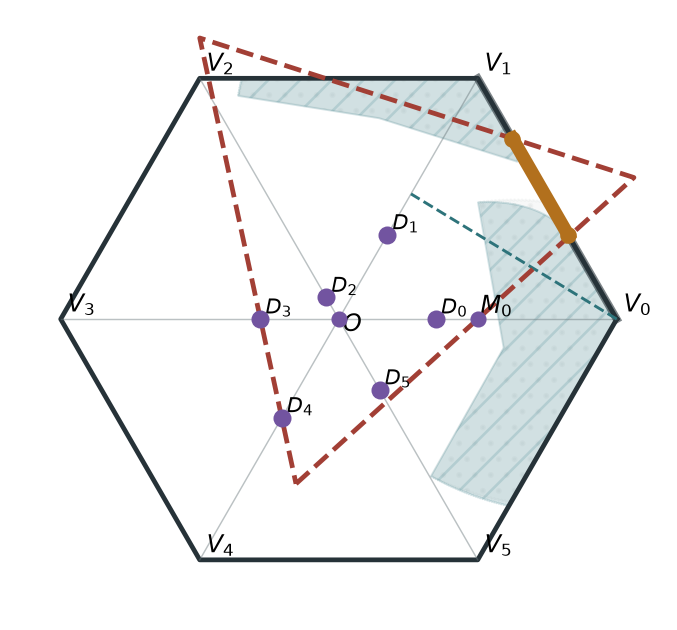
\includegraphics[width=\linewidth]
  {figures/trace_exact_ab/one_gap_n1_t3.png}
\par\smallskip
\textbf{One gap.}\par\smallskip
{\footnotesize
\(\begin{gathered}
N_{\rm gap}=1\\
N_+=1\\
(d,t)=(0,1)
\end{gathered}\)}
\end{minipage}\hfill
\begin{minipage}[t]{.485\linewidth}
\centering
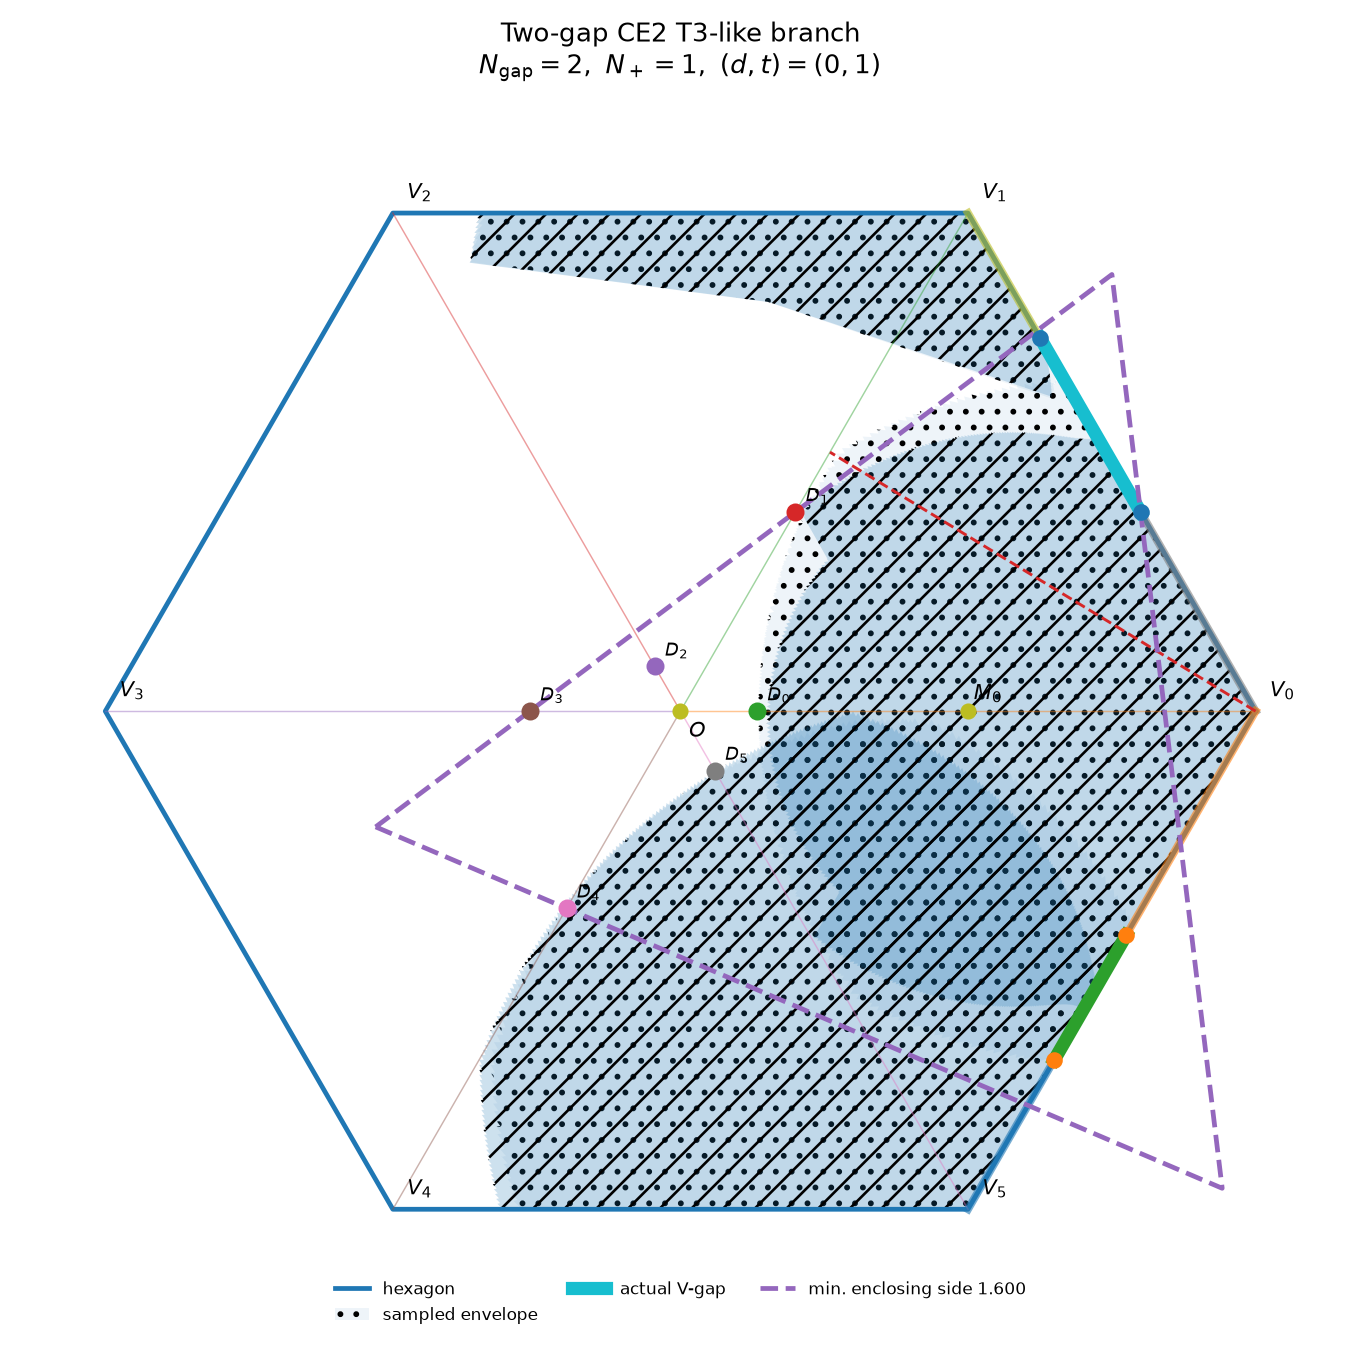
\includegraphics[width=\linewidth]
  {figures/trace_exact_ab/two_gap_n1_t3.png}
\par\smallskip
\textbf{Two gaps.}\par\smallskip
{\footnotesize
\(\begin{gathered}
N_{\rm gap}=2\\
N_+=1\\
(d,t)=(0,1)
\end{gathered}\)}
\end{minipage}
\caption{Case \(D_T\): sampled \(\Tlike\) supported-tail data.}
\label{fig:finite-enclosure-case-dt-examples}
\end{figure}

\FloatBarrier

For radial separation along \(r_i\), define
\[
 d_i^C:=\max\{x\in[0,1]:xV_i\in T_C\},
\]
\[
 c_{\rm loc}:=
 \sup\{s\in[0,1]:
 V_i+s(O-V_i)\in U_{i-1}\cup U_i\cup U_{i+1}\}.
\]
Then
\[
 T_C\cap r_i=\{xV_i:0\le x\le d_i^C\},
\]
\[
 (U_{i-1}\cup U_i\cup U_{i+1})\cap r_i
 \subseteq\{xV_i:1-c_{\rm loc}\le x\le1\}.
\]
Thus the exact strict inequality
\[
 c_{\rm loc}<1-d_i^C
\]
leaves the nonempty interval
\[
 \{xV_i:d_i^C<x<1-c_{\rm loc}\}
 \subseteq S\setminus
 \left(U_C\cup\bigcup_{j=0}^5U_j\right).
\]

For the nonadjacent adapter, if \(I\subseteq[0,1]\) is empty or a closed
interval, define
\[
 \mathcal R_I(p):=
 1-\sup\{x\in[0,1]:[0,x]\subseteq[0,p]\cup I\}.
\]
Put
\[
 I_R:=\{x\in[0,1]:X_0(x)\in T_C\},
 \qquad
 I_L:=\{x\in[0,1]:X_5(1-x)\in T_C\},
\]
\[
 \rho_R:=\mathcal R_{I_R}(B_0),
 \qquad
 \rho_L:=\mathcal R_{I_L}(A_0),
 \qquad
 \rho:=\min\{\rho_R,\rho_L\},
 \qquad
 D_\tau:=\rho V_\tau.
\]
Appendix D proves the exact separation inequalities for both adapters.

\subsection{The Vd placement router}

\begin{proposition}[Direct one-Vd placement assembly]
\label{prop:new-one-vd-assembly}
Assume
\[
 N_E(T_C)=2,
 \qquad
 N_{\rm gap}\in\{1,2\},
 \qquad
 N_+=1,
 \qquad
 (d,t)=(1,0),
\]
\[
 T_C\cap\{M_0,\ldots,M_5\}=\{M_0\}.
\]
Then the skeleton is not covered.
\end{proposition}

\begin{figure}[!htbp]
\centering
\begin{minipage}[t]{.485\linewidth}
\centering
\resizebox{.96\linewidth}{!}{%
\begin{tikzpicture}[x=6cm,y=1cm,>=Latex]
  \node[panellabel,anchor=west] at (-.02,2.28)
    {(a) adjacent Vd role: an uncovered interval on $r_2$};
  \draw[flow] (0,1.12)--(1,1.12);
  \fill (0,1.12) circle (.017) node[left=2pt,figlabel] {$V_2$};
  \fill (1,1.12) circle (.017) node[right=2pt,figlabel] {$O$};
  \coordinate (U) at (.46,1.12);
  \coordinate (C) at (.58,1.12);
  \coordinate (Q) at (.74,1.12);
  \draw[VertexOrange,line width=1.1pt] (0,1.19)--(U);
  \draw[RadialTeal,line width=1.1pt] (0,1.05)--(C);
  \draw[centertrace] (Q)--(1,1.12);
  \fill[VertexOrange] (U) circle (.021) node[above=3pt,figlabel] {$u_{1\to2}$};
  \fill[RadialTeal] (C) circle (.021) node[below=3pt,figlabel] {$C_2$};
  \fill[CenterBlue] (Q) circle (.022) node[above=3pt,figlabel] {$q_2=1-\delta$};
  \draw[gap] (C)--(Q);
  \fill[DemandRed] (.66,1.12) circle (.022)
    node[below=3pt,figlabel] {$Z_2$};
  \node[figlabel,align=center] at (.5,.10)
    {$u_{1\to2},C_2<q_2$; choose any $Z_2$ in the displayed interval\\
     coordinate is measured from $V_2$ toward $O$};
\end{tikzpicture}%
}
\end{minipage}\hfill
\begin{minipage}[t]{.485\linewidth}
\centering
\resizebox{.96\linewidth}{!}{%
\begin{tikzpicture}[x=6cm,y=1cm,>=Latex]
  \node[panellabel,anchor=west] at (-.02,2.28)
    {(b) nonadjacent Vd role: the residual-tail point};
  \draw[flow] (0,1.12)--(1,1.12);
  \fill (0,1.12) circle (.017) node[left=2pt,figlabel] {$O$};
  \fill (1,1.12) circle (.017) node[right=2pt,figlabel] {$V_\tau$};
  \coordinate (E) at (.23,1.12);
  \coordinate (Vd) at (.39,1.12);
  \coordinate (D) at (.56,1.12);
  \draw[centertrace] (0,1.12)--(E);
  \draw[actualreach] (1,1.12)--(Vd);
  \fill[CenterBlue] (E) circle (.022) node[above=3pt,figlabel] {$T=\alpha+\delta$};
  \fill[VertexOrange] (Vd) circle (.021) node[below=3pt,figlabel] {Vd endpoint};
  \fill[DemandRed] (D) circle (.024) node[above=3pt,figlabel] {$D_\tau$};
  \draw[gap] (E)--(D);
  \node[figlabel,align=center] at (.5,.10)
    {$T<\min\{\rho_R,\rho_L\}$ and\\
     $D_\tau=\min\{\rho_R,\rho_L\}V_\tau$ lies beyond both traces};
\end{tikzpicture}%
}
\end{minipage}

\vspace{.4em}

\begin{minipage}[t]{.485\linewidth}
\centering
\resizebox{.96\linewidth}{!}{%
\begin{tikzpicture}[x=6cm,y=1cm,>=Latex]
  \node[panellabel,anchor=west] at (-.02,2.28)
    {(c) Vd1 midpoint rescue};
  \draw[flow] (0,1.12)--(1,1.12);
  \fill (0,1.12) circle (.017) node[left=2pt,figlabel] {$V_1$};
  \fill (1,1.12) circle (.017) node[right=2pt,figlabel] {$O$};
  \coordinate (C) at (.23,1.12);
  \coordinate (M) at (.50,1.12);
  \coordinate (U) at (.72,1.12);
  \draw[actualreach] (C)--(U);
  \fill[CenterBlue] (M) rectangle +(0.025,0.025);
  \node[above=3pt,figlabel] at (M) {$M_1$};
  \draw[VertexOrange,fill=white,line width=.7pt] (U) circle (.025);
  \fill[DemandRed] (U) circle (.011);
  \node[above=3pt,figlabel] at (U) {$P_{\mathrm{Vd1}}$};
  \node[figlabel,align=center] at (.5,.10)
    {the same O-side endpoint mechanism as in the T3-like case;\\
     only the local normal-form inequality changes};
\end{tikzpicture}%
}
\end{minipage}\hfill
\begin{minipage}[t]{.485\linewidth}
\centering
\resizebox{.96\linewidth}{!}{%
\begin{tikzpicture}[x=1cm,y=1cm,>=Latex]
  \node[panellabel,anchor=west] at (-.05,2.35)
    {(d) two-chart replacement when both roles are away from $T_0$};
  \node[atlasbox,align=center,figlabel,text width=2.6cm]
    (old) at (1.45,1.12)
    {original Vd1--supercritical\\pair in one vertex chart};
  \node[atlasbox,align=center,figlabel,text width=2.6cm]
    (new) at (5.15,1.12)
    {two nonsupercritical Vd0\\roles in the correct charts};
  \node[atlasbox,align=center,figlabel,text width=2.6cm]
    (rank) at (8.85,1.12)
    {recompute $N'_{\rm gap}$:\\$0$, $1$, or $2$};
  \draw[flow] (old)--node[above,figlabel] {replace} (new);
  \draw[flow] (new)--node[above,figlabel] {do not preserve input rank} (rank);
  \node[figlabel,align=center] at (8.85,.08)
    {$0$: trace length\qquad$1$: disk--gap\qquad$2$: short ray};
\end{tikzpicture}%
}
\end{minipage}
\caption{The four geometric terminals in the one-Vd placement assembly.
In the adjacent placement the radial coordinate is measured from $V_2$
toward $O$; the two local V endpoints lie before the center interval entry
$q_2=1-\delta$, leaving a literal uncovered interval on $r_2$.  The
nonadjacent placement produces the point
$D_\tau=\min\{\rho_R,\rho_L\}V_\tau$ beyond both the Vd and center traces;
the Vd1 midpoint rescue uses the same O-side endpoint construction as the
T3-like case; and the remaining placement is reduced by a two-chart
replacement followed by recomputation of the output gap rank.  Lengths are
schematic; all labelled order relations are the proof relations.}
\label{fig:one-vd-placement-terminals}
\end{figure}


\begin{proof}
If \(\sigma=0\) and \(\tau\in\{1,5\}\), the adjacent radial-separation
calculation gives \(c_{\rm loc}<1-d_2^C\) on \(r_2\).  If
\(\sigma=0\) and \(\tau\in\{2,3,4\}\), the nonadjacent calculation gives
\[
 d_\tau^C<\rho<1-C_\tau,
 \qquad
 D_\tau\in
 S\setminus\left(U_C\cup\bigcup_{j=0}^5U_j\right).
\]
If the Vd role is based at \(T_0\), Vd2 closes by the trace bound and Vd1
closes by the supported-tail adapter.  These three calculations are in
\zcref{lem:appendix-adjacent-vd-separation,
lem:appendix-nonadjacent-vd-separation,
lem:appendix-vd1-supported-tail}.

It remains that \(\sigma,\tau\ne0\).  Midpoint rescue makes the two roles
adjacent.  Vd2 again closes by trace length.  For Vd1, fresh cyclic
renumbering and reflection give \((\tau,\sigma)=(0,1)\), with
\[
 (o(T_0),n(T_0))=(1,1),
 \qquad
 A_0+B_0<\frac12,
 \qquad
 M_1\in T_0,
 \qquad
 A_1+B_1>1,
\]
\[
 A_i+B_i\le1\quad(i\ne1),
\]
\[
 (o(T_i),n(T_i))\in\{(1,0),(2,0)\}
 \quad(1\le i\le5),
\]
\[
 U_C\cap e_{0,1}=\varnothing,
 \qquad
 \Haus(T_j\cap r_k)=0
 \quad(2\le j\le5,\ k\in\{0,1\}).
\]
The two-chart construction in
\zcref{prop:appendix-vd1-two-chart-replacement} produces
\(\varepsilon>0\) and open unit triangles \(U'_0,U'_1\), with \(V_k\in U'_k\),
such that, after
\[
 U'_i:=U_i\quad(2\le i\le5),
 \qquad
 T'_i:=\overline{U'_i}\quad(0\le i\le5),
\]
one has
\[
 S\subseteq U_C\cup\bigcup_{i=0}^5U'_i,
 \qquad
 (o(T'_i),n(T'_i))\in\{(1,0),(2,0)\}\quad(0\le i\le5),
\]
\[
 A(T'_i)+B(T'_i)\le1\quad(0\le i\le5),
\]
\[
 A(T'_0)+B(T'_0)=A(T'_1)+B(T'_1)=1-\varepsilon<1,
\]
where
\[
 A(T'_i):=\max\{x\in[0,1]:V_i+x(V_{i-1}-V_i)\in T'_i\},
\]
\[
 B(T'_i):=\max\{x\in[0,1]:V_i+x(V_{i+1}-V_i)\in T'_i\}.
\]
\[
 C(T'_i):=\max\{x\in[0,1]:V_i+x(O-V_i)\in T'_i\}.
\]
For the unchanged roles,
\[
 \bigl(A(T'_i),B(T'_i),C(T'_i)\bigr)=(A_i,B_i,C_i)
 \qquad(2\le i\le5).
\]
Moreover,
\[
 \left|\left\{i\in\mathbb Z/6\mathbb Z:
 A(T'_i)+B(T'_i)>1\right\}\right|=0.
\]
Define, from the output open traces,
\[
 N'_{\rm gap}:=
 \left|\left\{i\in\mathbb Z/6\mathbb Z:
 e_{i,i+1}\setminus
 \bigl((U'_i\cap e_{i,i+1})\cup(U'_{i+1}\cap e_{i,i+1})\bigr)
 \ne\varnothing\right\}\right|.
\]
Then \(N'_{\rm gap}\in\{0,1,2\}\).  If it is zero,
\zcref{prop:length-branches} applies.  If it is one, apply
\zcref{lem:new-one-gap-common-pair-adapter} to the primed actual reaches and
then the row-A branch of \zcref{prop:new-nplus-zero-gap-closures}.  If it is
two, apply
\zcref{lem:new-two-gap-common-pair-adapter} to the primed actual reaches and
then the row-B branch of \zcref{prop:new-nplus-zero-gap-closures}.  Thus the
common-pair hypotheses are rederived after replacement; the input and output
gap ranks are not asserted to be equal.
\end{proof}

\begin{figure}[!htbp]
\centering
\begin{minipage}[t]{.485\linewidth}
\centering
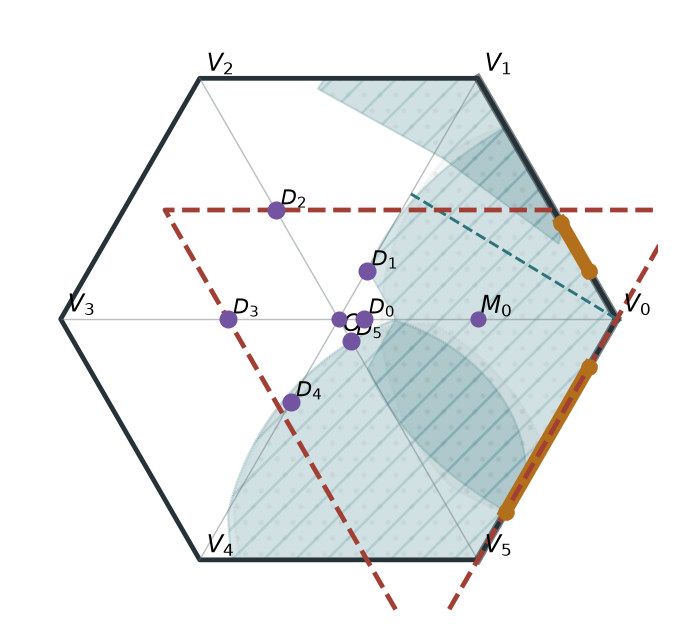
\includegraphics[width=\linewidth]
  {figures/trace_exact_ab/vd1_rescuer.png}
\par\smallskip
\textbf{\(\Vdone\) supported tail.}\par\smallskip
{\footnotesize
\(\begin{gathered}
N_{\rm gap}=2\\
N_+=1\\
(d,t)=(1,0)\\
(\sigma,\tau)=(1,0)\\
(o(T_0),n(T_0))=(1,1)\\
A_0+B_0<1/2
\end{gathered}\)}
\end{minipage}\hfill
\begin{minipage}[t]{.485\linewidth}
\centering
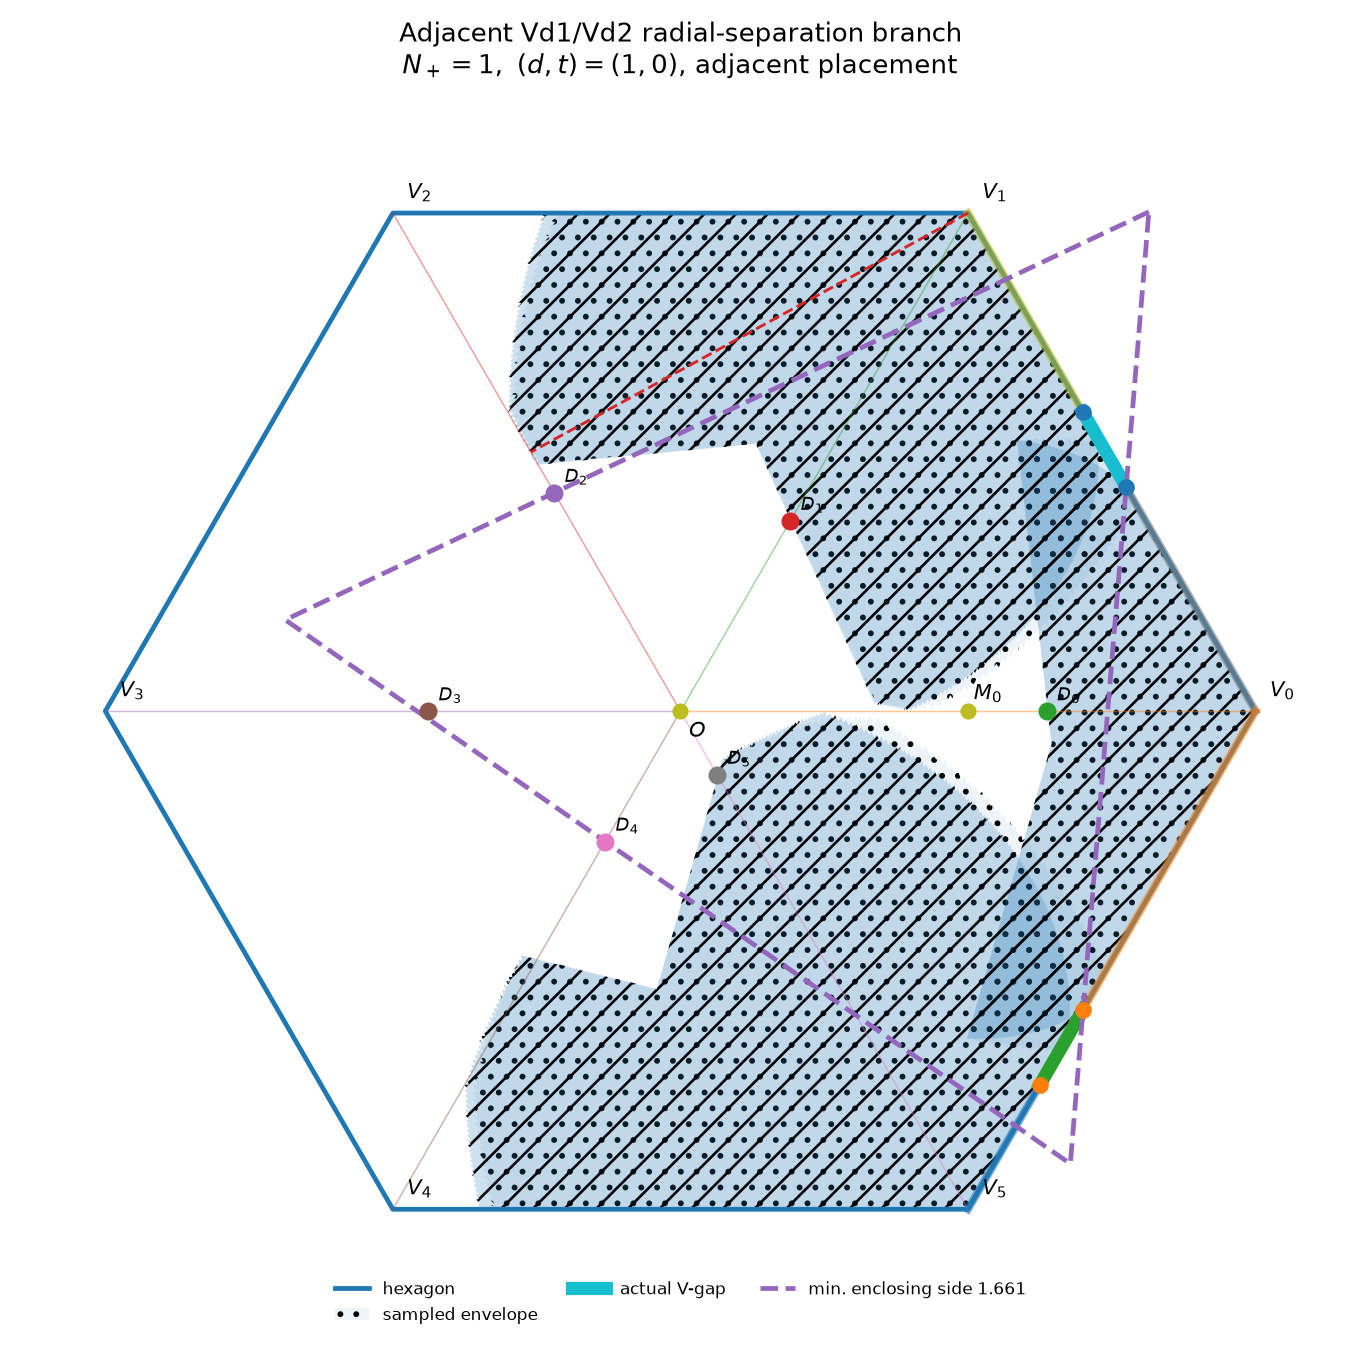
\includegraphics[width=\linewidth]
  {figures/trace_exact_ab/adjacent_vd.png}
\par\smallskip
\textbf{Adjacent separation.}\par\smallskip
{\footnotesize
\(\begin{gathered}
N_{\rm gap}=2\\
N_+=1\\
(d,t)=(1,0)\\
(\sigma,\tau)=(0,1)
\end{gathered}\)}
\end{minipage}

\par\medskip
\begin{minipage}[t]{.485\linewidth}
\centering
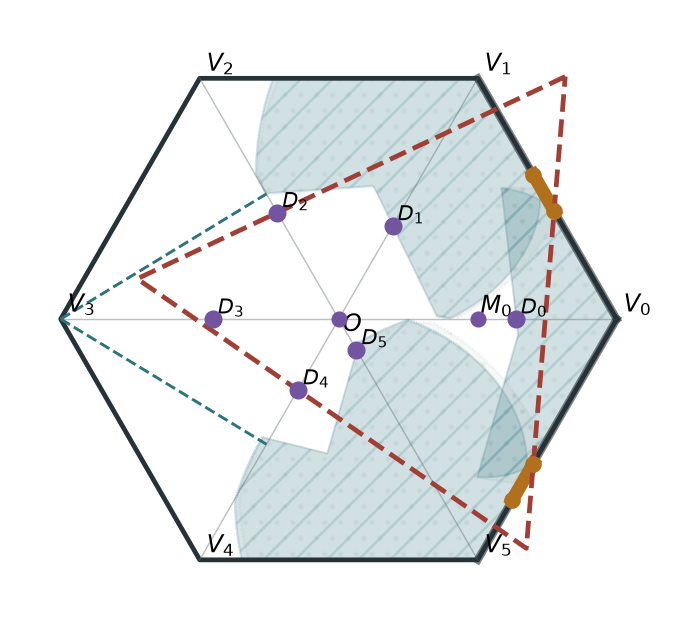
\includegraphics[width=\linewidth]
  {figures/trace_exact_ab/nonadjacent_vd.png}
\par\smallskip
\textbf{Nonadjacent separation.}\par\smallskip
{\footnotesize
\(\begin{gathered}
N_{\rm gap}=2\\
N_+=1\\
(d,t)=(1,0)\\
(\sigma,\tau)=(0,3)
\end{gathered}\)}
\end{minipage}\hfill
\begin{minipage}[t]{.485\linewidth}
\centering
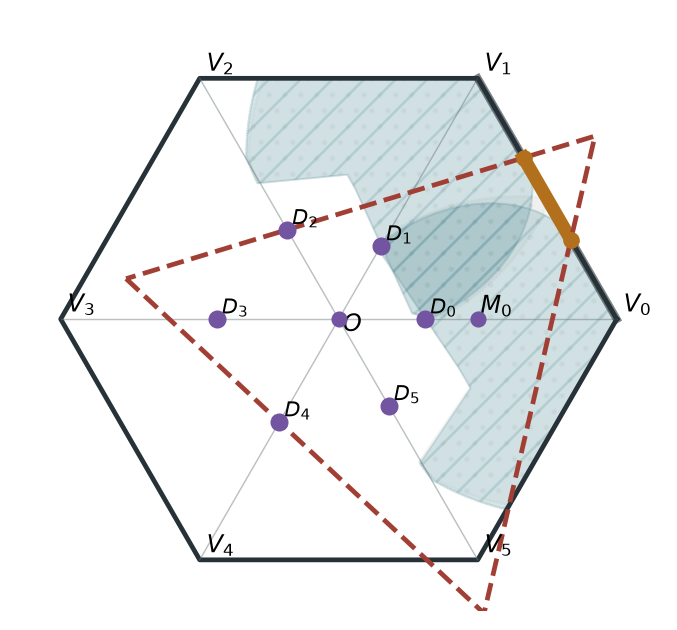
\includegraphics[width=\linewidth]
  {figures/trace_exact_ab/replacement_output.png}
\par\smallskip
\textbf{Replacement output \(R\to A\).}\par\smallskip
{\scriptsize
\(\begin{gathered}
N'_{\rm gap}=1\\
A(T'_i)+B(T'_i)\le1\quad(i\in\mathbb Z/6\mathbb Z)\\
(o(T'_i),n(T'_i))\in\{(1,0),(2,0)\}
\quad(i\in\mathbb Z/6\mathbb Z)
\end{gathered}\)}
\end{minipage}
\caption{Cases \(D_V\), \(E_a\), \(E_n\), and R: sampled
router data.}
\label{fig:finite-enclosure-vd-router-examples}
\end{figure}

\FloatBarrier

\begin{proposition}[All nonzero-gap finite-enclosure rows]
\label{prop:finite-enclosure-nonzero-gap-branches}
Every nonzero-gap row of \zcref{tab:routing} assigned to finite enclosure is
impossible.
\end{proposition}

\begin{proof}
Rows A and B are \zcref{prop:new-nplus-zero-gap-closures}; row C is
\zcref{prop:new-nplus-one-all-vd0}; and rows D, E, and R are
\zcref{prop:new-one-t3-terminal,prop:new-one-vd-assembly}.
\end{proof}
